% !TeX spellcheck = en_US
% Chapter Template

\chapter{Background and related work} % Main chapter title

\label{chap:background} % Change X to a consecutive number; for referencing this chapter elsewhere, use \ref{ChapterX}

\lhead{Chapter \ref*{chap:background}. \emph{Background and related work}} % Change X to a consecutive number; this is for the header on each page - perhaps a shortened title

\section{Application under study}
\ac{OT} is a open-source simulation platform developed by the university of Applied Sciences in Frankfurt, Germany. It covers features like computer aided design, 3D modeling, meshing, and flow and physics simulation (like FIT-TD and PHREEC). The projects can be administered by a user and group management (see~\autoref{fig:ot-project}). Furthermore, all changes on a project are version-controlled. The application is designed in a way, that only a local thin-client needs to run on the users computer. After entering the login credentials (see~\autoref{fig:ot-login}), the client securely connects to a centralized service platform where the computation is made. The results and even the \ac{UI} information is sent back to the client application. This has the benefit, that also weak computers can run the application. 

\begin{figure}[h]
	\centering
	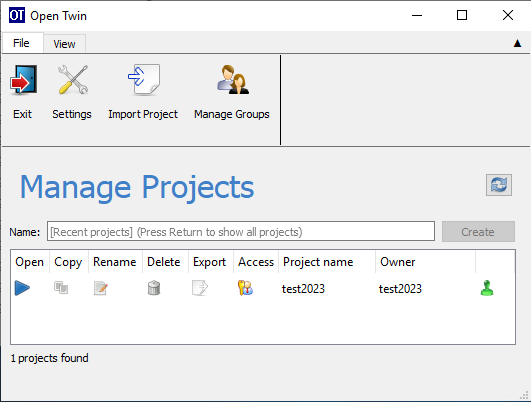
\includegraphics[width=.9\textwidth]{Figures/ot-project.png}
	\caption{The \ac{OT} project overview.}
	\label{fig:ot-project}
\end{figure}

\begin{figure}[h]
	\centering
	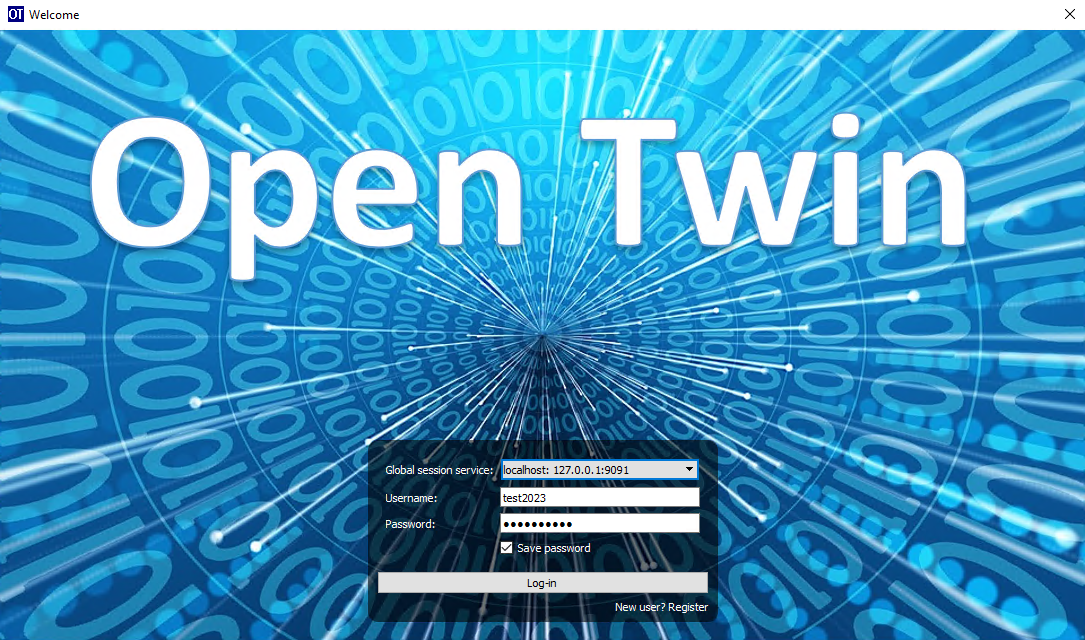
\includegraphics[width=.9\textwidth]{Figures/ot-login.png}
	\caption{The \ac{OT} login screen.}
	\label{fig:ot-login}
\end{figure}

\autoref{fig:ot-model} shows the application itself with a loaded project and a simple geometric model.
\begin{figure}[h]
	\centering
	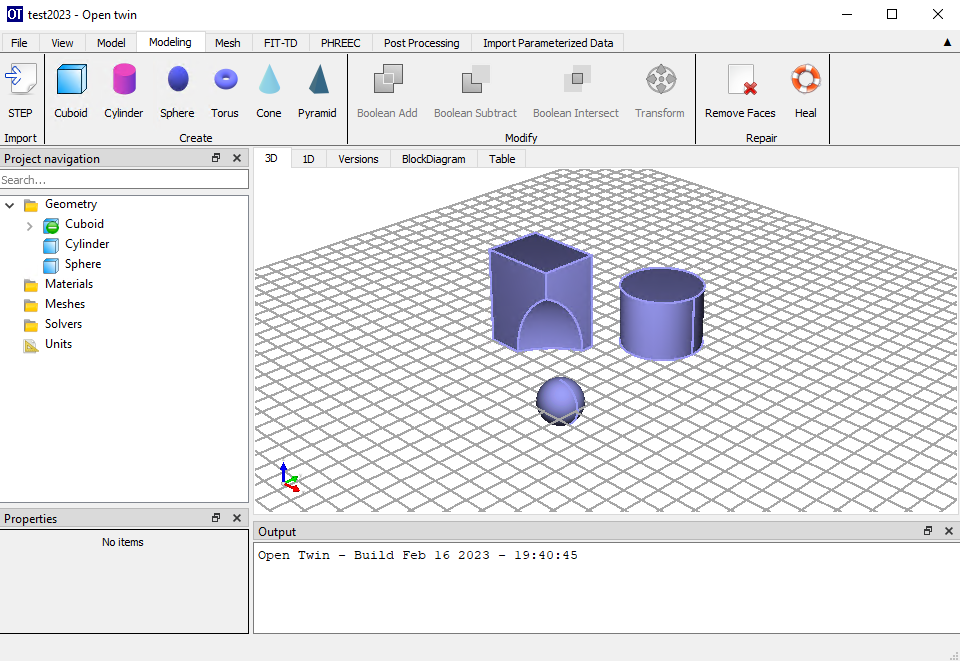
\includegraphics[width=.9\textwidth]{Figures/ot-model.png}
	\caption{A opened project inside \ac{OT} with a few created geometric models and subtracted computation.}
	\label{fig:ot-model}
\end{figure}

The development team consists of a small core team and several student groups during the semester.


\section{Baseline architecture}
The current system design consists of multiple levels. It is a multi-process application based on the programming languages C++ and Rust. The source code is mainly aligned to be built on Microsoft \ac{Windows}. A port to Unix based systems is currently in work. Therefore parts of the code base are aligned for multiple system architectures already, but the application is not yet able to be compiled for Linux.

Each microservice of the application is included dynamically and linked as a \ac{DLL} file. For starting the microservice environment, a central executable ("open\_\ twin.exe") is started with the corresponding arguments for the services (like binding address, port numbers, encrypted passwords) (see~\autoref{lst:ot-command}) and the path to the \ac{DLL} file itself. The UI frontend, which is started by the user directly, is compiled in its own executable ("uiFrontend.exe"). \autoref{tbl:ot-command-args} shows the main services and its corresponding parameters.

\begin{lstlisting}[language=sh, caption={Command line of Open Twin Service start}, label=lst:ot-command]
open_twin.exe GlobalSessionService.dll \
  "0" "127.0.0.1:8091" "tls@127.0.0.1:27017" "127.0.0.1:8092"
\end{lstlisting}

\begin{table}[h!]
	\centering
	\begin{tabular}{||c c c c||} 
		\hline
		Col1 & Col2 & Col2 & Col3 \\ [0.5ex] 
		\hline\hline
		1 & 6 & 87837 & 787 \\ 
		2 & 7 & 78 & 5415 \\
		3 & 545 & 778 & 7507 \\
		4 & 545 & 18744 & 7560 \\
		5 & 88 & 788 & 6344 \\ [1ex] 
		\hline
	\end{tabular}
	\caption{Table to test captions and labels.}
	\label{tbl:ot-command-args}
\end{table}

For conveniently running the services with all their necessary arguments, batch files were provided that read environment variables and convert them into runtime arguments for the service executable. Therefore, if the services are started locally, the user runs a batch files that sets up the environment.

The system consists of the following microservices that are permanently accessible: \ac{GSS}, \ac{AUTH} and the database. The database is running on MongoDB\footnote{MongoDB:~https://www.mongodb.com/}. Another Service is the \ac{LSS} that spawns the so called application services. Those are services for logging, scripting, 3D modeling, kriging and so on.
While \ac{GSS}, \ac{AUTH} and database are globally accessible, the \ac{LSS} can theoretically run on a dedicated host and is only communicated to other parties after it has registered itself to the \ac{GSS}.

Once started, the user can login. In order to connect to the database, the following steps are performed:
\begin{enumerate}
\item The \ac{UI} frontend requests further service information from the \ac{GSS}. It responses with \acp{URL} to the database and the \ac{AUTH}.
\item The \ac{UI} frontend connects to the \ac{AUTH} using the authentication information provided by the user.
\item If the \ac{AUTH} replies with a positive authentication, the \ac{UI} frontend connects to the database and lists the projects.
\item Once a project is opened or created, the \ac{UI} frontend requests a new session from the \ac{GSS}. The \ac{GSS} replies with the connection \acp{URL} from the \ac{LSS}. The \ac{LSS} has been registered to the \ac{GSS} during its initialization.
\item The \ac{UI} frontend then connects to the \ac{LSS} and requests a new session. As a result, the \ac{LSS} spawns new application service processes and replies with the respective service \acp{URL}.
\item From now on, the \ac{UI} frontend communicates with the application services.
\end{enumerate}
The whole process of the \ac{LSS} registration and connection of the \ac{UI} frontend to the compute services is depicted in \autoref{fig:ot-network-communication}.

\begin{figure}[h]
	\centering
	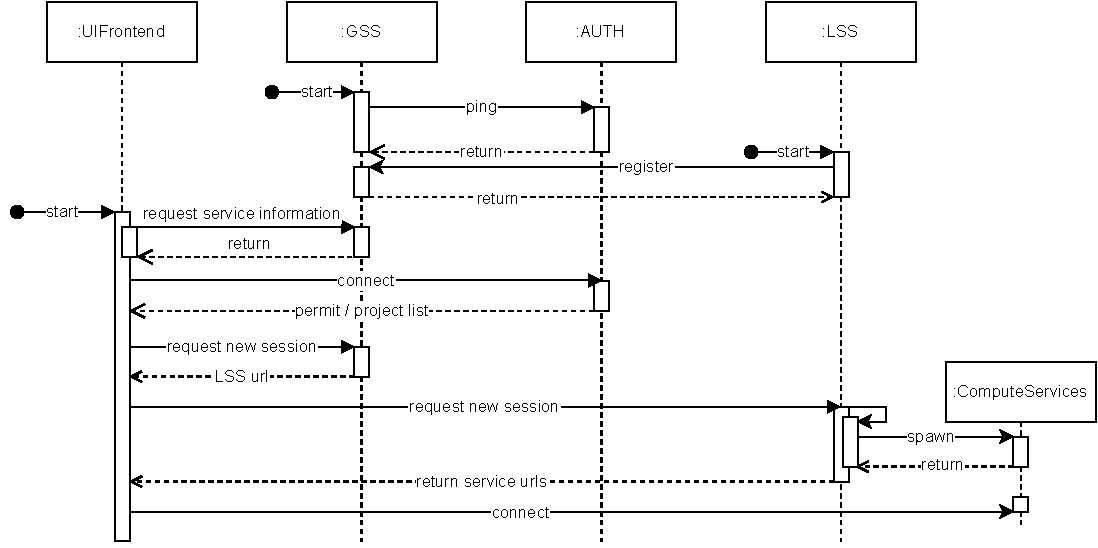
\includegraphics[width=0.98\textwidth]{Figures/opentwin-network-communication.pdf}
	\caption{Service initialization of OpenTwin processes. (Ping messages are omitted.)}
	\label{fig:ot-network-communication}
\end{figure}

The traffic between services is encrypted using \ac{mTLS} technology. While regular \ac{TLS} ensures the authenticity of the server by using Certificates and the chain of trust, it does not verify the identity of the client. This is the benefit of \ac{mTLS}. In \ac{mTLS}, both sides, client and server has to verify their identity by providing a certificate inherited from a common root certificate.

\section{Problem statement}
Even though, the application is clearly based on a microservice architecture and it is able to run on a distributed system, it is not designed for a automated cluster yet. It consists of multiple processes where many of them have to run on the same system and need a full working operating system as baseline. Containerization of the system has never been tested and needs to be introduced. 
First, the cluster engine needs to be set up for \ac{Windows} compute nodes to allow \ac{Windows} containers to run inside the cluster. Additionally, it needs to have full network capabilities as well as inter connectivity between the several services.
Next, the application needs to run inside containers. Therefore, container images must be created and provided for the cluster engine. 
Additionally, the automatic extension of services requires communication between the cluster orchestration management and the applications running on the nodes. A feature that needs to be introduced later on.

Regarding logging, while the frontend application does, the microservices currently do not produce log files. Instead, only a few sub processes write the information on its standard output stream. In some cases, the error information given by exceptions is dropped.
Furthermore, proper exit codes in error cases are not returned. That is, if the application exits there is currently no way to detect if the process terminated normally or crashed as part of an error.

\section{Limitations}
Due to the limited amount of time, not all code changes are applied. On the one hand, this involves the adaption for automatic extension of services. On the other hand, it implies the changes required to make the application more fault-tolerant. The changes that would be necessary, would be too extensive. Therefore, they are only made to the main processes.

As a first case study, the application is not fully containerized. Since the network connectivity is known to cause troubles in \ac{Windows} container networks, there is more investigation required later on. As part of this study, only the main services are containerized and the cluster is set up to investigate the behavior in cluster environments. The actual distribution of an full functional cluster network can be part of further studies later on.

\section{Related Work}
